%packages
  %layout

\documentclass[10pt,a4paper]{scrartcl} %scrartcl from KOMA-script uses sans headers and looks less latexy than article  \usepackage[doublespacing]{setspace}
  \usepackage[utf8]{inputenc}
  \usepackage[doublespacing]{setspace}
  \usepackage[left=2.5cm,right=2.5cm,top=3cm,bottom=3cm]{geometry}
  \usepackage{subcaption}
  \usepackage{adjustbox}
  \usepackage{tabularx}
  %\usepackage{blindtext,titlefoot}

  %graphics, equations and math 
  \usepackage{amsmath}
  \usepackage{graphicx}
  \usepackage{pdfpages}


  %tables
  \usepackage{tabularx}
  \usepackage{threeparttable}
  \usepackage{csvsimple}
  \usepackage{booktabs}

  %bibliography and references
  \usepackage{natbib}
  \usepackage{url}
  \usepackage[pdftex, hidelinks]{hyperref} %creates warnings when used with float

%special cell that allows line breaks
\newcommand{\specialcell}[2][c]{%
  \begin{tabular}[#1]{@{}c@{}}#2\end{tabular}}

\begin{document}
\author{Koen Leuveld}




\title{Comparison Tables }
%\subtitle{Exploratory evidence from a list experiment in Eastern DR Congo} %needs scrartcl

\maketitle

\begin{figure}
  \begin{center}
    \caption{Figure 1 Cannot be replicated using anonymized data} \label{fig:slf:conflictexposure}
  \end{center}
\end{figure}

%tables
%\begin{adjustbox}{totalheight=\textheight-2\baselineskip}
\begin{table}
  \begin{threeparttable}
    \caption{Descriptive Statistics}
    \label{tab:slf:summstats}
    \renewcommand{\arraystretch}{0.6}
    % \tiny 
    % \scriptsize
    %\footnotesize
    % \small
    % \normalsize
    {
\def\sym#1{\ifmmode^{#1}\else\(^{#1}\)\fi}
\begin{tabular}{l*{1}{ccccc}}
\hline\hline
                    &\multicolumn{5}{c}{}                                            \\
                    &       count&        mean&          sd&         min&         max\\
\hline
Exposure to conflict&         162&        0.57&        0.26&        0.00&        1.00\\
Parent fought in war&         162&        0.12&        0.33&        0.00&        1.00\\
Age                 &         162&       19.75&        3.44&       14.00&       31.00\\
Education Level     &         162&        2.64&        0.75&        1.00&        4.00\\
Meals per day       &         162&        2.44&        0.63&        1.00&        3.00\\
Muslim              &         162&        0.79&        0.41&        0.00&        1.00\\
Mende               &         162&        0.54&        0.50&        0.00&        1.00\\
Fula                &         162&        0.16&        0.37&        0.00&        1.00\\
Mandingo            &         162&        0.11&        0.32&        0.00&        1.00\\
Temne               &         162&        0.07&        0.26&        0.00&        1.00\\
Always in Kenema    &         162&        0.52&        0.50&        0.00&        1.00\\
Foul card           &         162&        0.20&        0.40&        0.00&        1.00\\
Played whole game   &         162&        0.46&        0.50&        0.00&        1.00\\
Self-declared skills&         162&        0.86&        0.23&        0.00&        1.00\\
Scored              &         162&        0.17&        0.38&        0.00&        1.00\\
Won the football game&         162&        0.42&        0.50&        0.00&        1.00\\
Left footed         &         162&        0.19&        0.39&        0.00&        1.00\\
Risk Preferences    &         162&        0.00&        1.00&       -1.56&        1.19\\
0 life\_dict         &         162&       -0.27&        1.09&       -3.43&        2.39\\
1 life\_dict         &         162&        0.27&        0.81&       -2.70&        3.84\\
Outgroup Tournament &          70&        0.43&        0.50&        0.00&        1.00\\
Ingroup Tournament  &          92&        0.41&        0.50&        0.00&        1.00\\
Expected performance&         162&        0.91&        0.13&        0.60&        1.00\\
Balls on target     &         162&        6.27&        1.82&        1.00&       10.00\\
\hline\hline
\end{tabular}
}

    \begin{tablenotes}
      \footnotesize
      \item \textit{Notes:} See Appendix I for variable definitions.
    \end{tablenotes}
   \end{threeparttable}
\end{table}
%\end{adjustbox}

\begin{figure}
  \begin{center}
    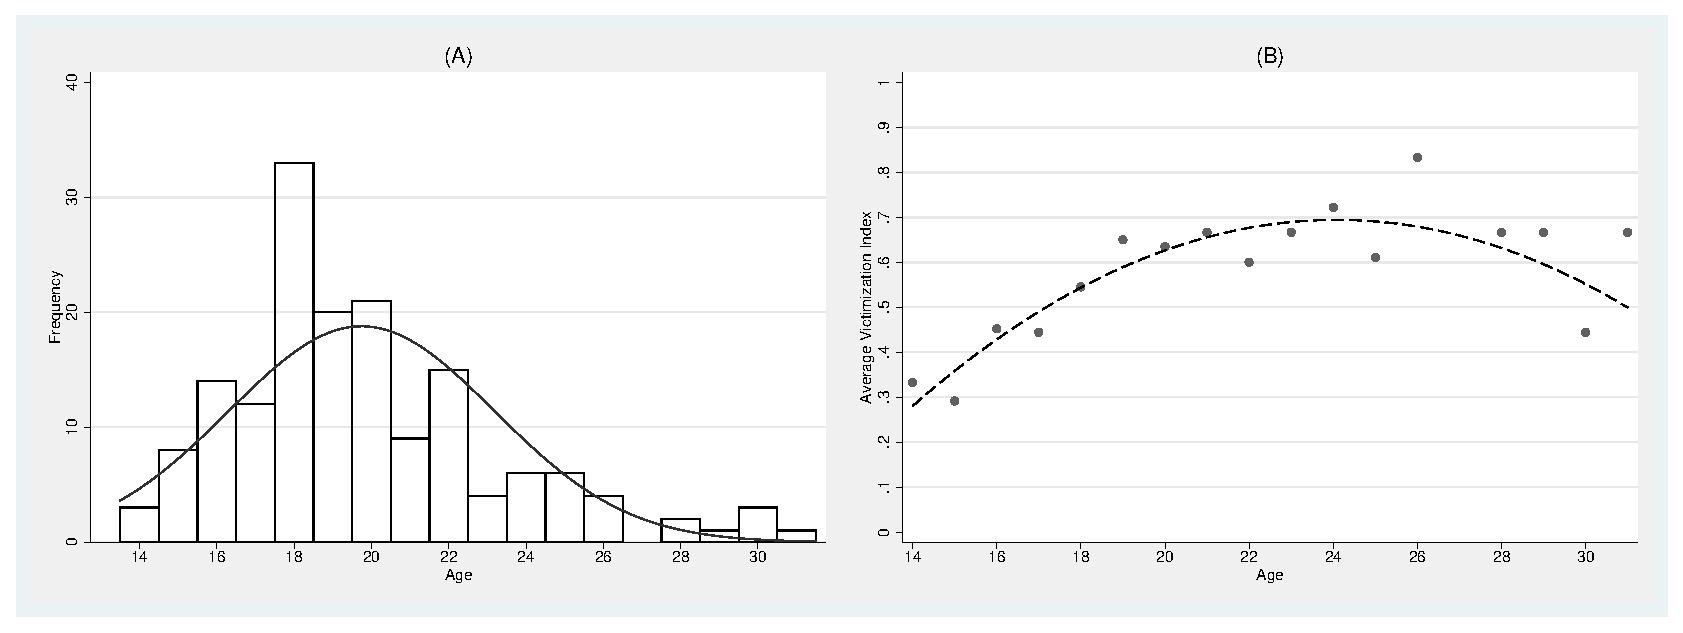
\includegraphics[width=\linewidth]{"Outputs_anon/figures/f2_agefreq_agewe.eps"}
    \caption{Age in sample and exposure to conflict}
    \label{fig:slf:ageconflict}
    \subcaption*{\textit{Notes:} panel A shows the distribution of age in our sample. Panel B shows the relationship between age and victimization index.}
  \end{center}
\end{figure}

\begin{figure}
  \begin{centering}
    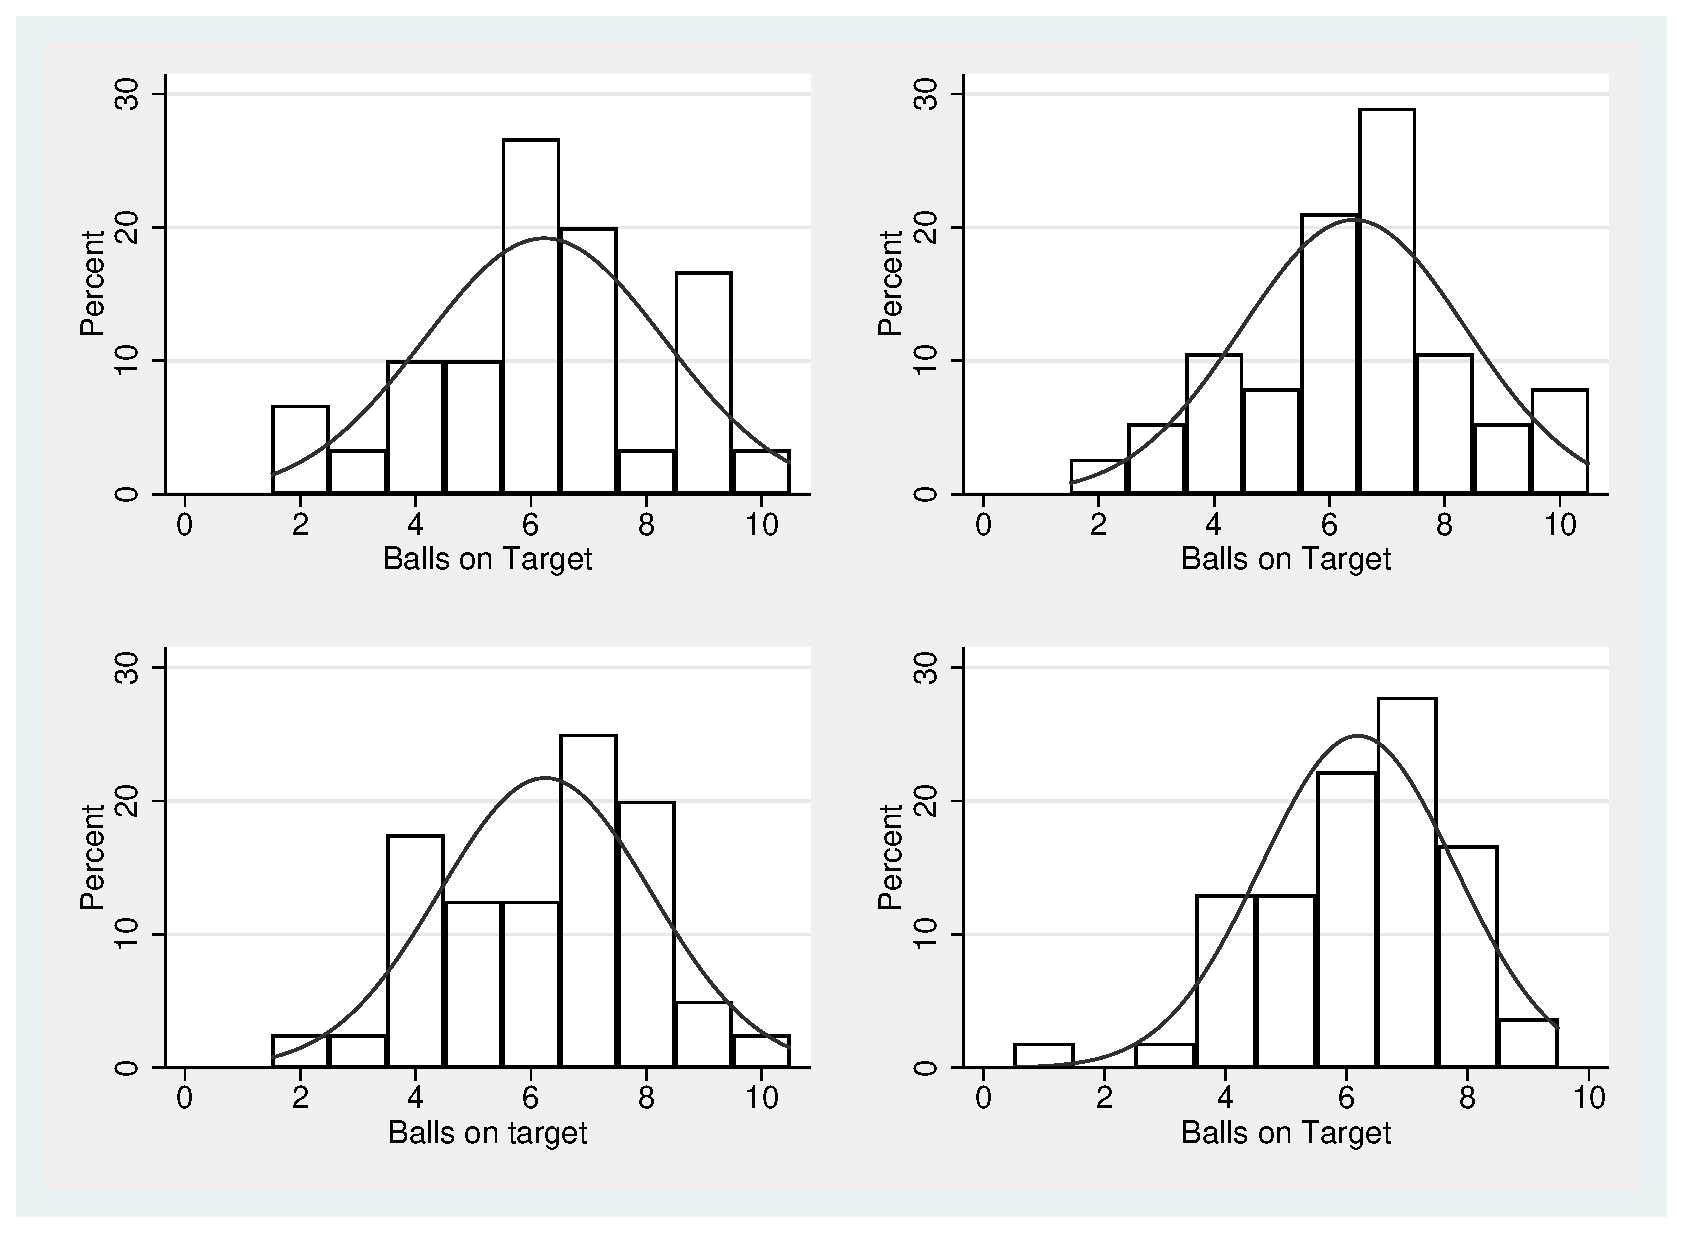
\includegraphics[width=0.6\linewidth]{"Outputs_anon/figures/f3_ballshit.eps"}
    \caption{Balls hit in the effort game}
    \label{fig:slf:ballshit}
    \subcaption*{\textit{Notes:} distribution of number of balls hit for four subsamples: Panel A: Out-group, opted for tournament; Panel B: In-group opted for tournament; C: Out-group, did not opt for tournament; D: In-group, did not opt for tournament }
  \end{centering}
\end{figure}

\begin{table}
  \centering
  \begin{threeparttable}
  \singlespacing
  \caption{Risk Propensity Game Choice Sets}
  \begin{tabular}{cccc}
    \toprule
          & \multicolumn{2}{c}{Coin Toss} &  \\
    Choice set & If heads & If tails & For certain \\
    \midrule
    1    & 3000  & 0     & 100 \\
    2    & 3000  & 0     & 500 \\
    3    & 3000  & 0     & 1000 \\
    4    & 3000  & 0     & 1500 \\
    5    & 3000  & 0     & 2000 \\
    6    & 3000  & 0     & 2500 \\
    \bottomrule
  \end{tabular}%
  \begin{tablenotes}
    \item \textit{Notes:} monetary amounts are reported in Leones. The exchange rate at the time of data collection was about 4400 Leones to 1 USD.
    \item
  \end{tablenotes}
  \label{tab:sl:riskchoice}%
  \end{threeparttable}%
\end{table}

\begin{table}
  \centering
  \begin{threeparttable}[p!]
    \caption{Exposure to Conflict}
    \singlespacing
    %\setlength\extrarowheight{-10pt}
    %\renewcommand{\arraystretch}{0.6}
    % \tiny 
    % \scriptsize
    %\footnotesize
    \small
    % \normalsize
    \label{tab:slf:conflictexposure}
    {
\def\sym#1{\ifmmode^{#1}\else\(^{#1}\)\fi}
\begin{tabular}{l*{4}{c}}
\hline\hline
                    &\multicolumn{1}{c}{(1)}         &\multicolumn{1}{c}{(2)}         &\multicolumn{1}{c}{(3)}         &\multicolumn{1}{c}{(4)}         \\
\hline
20-24               &       0.126\sym{***}&       0.123\sym{***}&       0.125\sym{***}&       0.105\sym{**} \\
                    &    (0.0415)         &    (0.0420)         &    (0.0416)         &    (0.0500)         \\
[1em]
25-29               &       0.173\sym{***}&       0.159\sym{**} &       0.169\sym{***}&       0.144\sym{*}  \\
                    &    (0.0569)         &    (0.0633)         &    (0.0552)         &    (0.0741)         \\
[1em]
30-34               &       0.145\sym{***}&                     &       0.154\sym{***}&                     \\
                    &    (0.0305)         &                     &    (0.0310)         &                     \\
[1em]
Muslim              &                     &     -0.0522         &                     &     -0.0273         \\
                    &                     &    (0.0522)         &                     &    (0.0622)         \\
[1em]
ind\_mende           &                     &       0.111\sym{**} &                     &       0.102\sym{**} \\
                    &                     &    (0.0427)         &                     &    (0.0453)         \\
[1em]
ind\_alwaysken       &                     &                     &                     &      0.0265         \\
                    &                     &                     &                     &    (0.0457)         \\
[1em]
ind\_edu             &                     &                     &                     &      0.0348         \\
                    &                     &                     &                     &    (0.0472)         \\
[1em]
Meals per day       &                     &                     &                     &     -0.0475         \\
                    &                     &                     &                     &    (0.0305)         \\
[1em]
Left footed         &                     &                     &                     &      0.0655         \\
                    &                     &                     &                     &    (0.0657)         \\
[1em]
Played whole game   &                     &                     &                     &     -0.0101         \\
                    &                     &                     &                     &    (0.0451)         \\
[1em]
Self-declared skills&                     &                     &                     &      0.0781         \\
                    &                     &                     &                     &    (0.0934)         \\
[1em]
Scored              &                     &                     &                     &    -0.00688         \\
                    &                     &                     &                     &    (0.0670)         \\
[1em]
Won the football game&                     &                     &                     &      0.0102         \\
                    &                     &                     &                     &    (0.0462)         \\
[1em]
Parent fought in war&                     &                     &      0.0723         &      0.0599         \\
                    &                     &                     &    (0.0596)         &    (0.0639)         \\
[1em]
Constant            &       0.522\sym{***}&       0.507\sym{***}&       0.513\sym{***}&       0.425\sym{**} \\
                    &    (0.0305)         &    (0.0628)         &    (0.0310)         &     (0.165)         \\
\hline
N                   &         150         &         142         &         150         &         141         \\
R2                  &       0.072         &       0.133         &       0.081         &       0.173         \\
\hline\hline
\end{tabular}
}

    \begin{tablenotes}
      \footnotesize
      \item \textit{Notes:} Ordinary Least Squares regressions. Robust standard errors in parentheses. Column 1 reports the marginal effect of age and age squared on exposure to conflict related violence (as measured by the individual victimization index, see Appendix I for variable definitions). Column 2 adds individual controls. Column 3 tests for the effect of active parental belligerence at any moment and for any faction during the civil war. Column 4 includes education, number of meals per day, and a series of football related variables as additional controls.  * p $<$ 0.10, ** p $<$ 0.05, *** p $<$ 0.01.
      \item
    \end{tablenotes}
\end{threeparttable}
\end{table}

\begin{table}
\centering
\begin{threeparttable}
  \caption{Aggressiveness and Risk Propensity}
  \label{tab:slf:aggrisk}
  \singlespacing
  %\renewcommand{\arraystretch}{0.6}
  % \tiny 
  % \scriptsize
  %\footnotesize
  % \small
  % \normalsize
  {
\def\sym#1{\ifmmode^{#1}\else\(^{#1}\)\fi}
\begin{tabular}{l*{4}{c}}
\hline\hline
                    &\multicolumn{1}{c}{(1)}&\multicolumn{1}{c}{(2)}&\multicolumn{1}{c}{(3)}&\multicolumn{1}{c}{(4)}\\
                    &\multicolumn{1}{c}{\specialcell{Foul\\Card}}&\multicolumn{1}{c}{\specialcell{Foul\\Card}}&\multicolumn{1}{c}{\specialcell{Risk\\Propensity}}&\multicolumn{1}{c}{\specialcell{Risk\\Propensity}}\\
\hline
main                &                     &                     &                     &                     \\
War Exposure        &       0.266\sym{**} &       0.378\sym{***}&       0.579\sym{**} &       0.539         \\
                    &     (0.125)         &     (0.132)         &     (0.281)         &     (0.341)         \\
[1em]
ind\_age==20-24 (d)  &                     &     -0.0938         &                     &       0.414\sym{*}  \\
                    &                     &    (0.0642)         &                     &     (0.220)         \\
[1em]
ind\_age==25-29 (d)  &                     &      -0.111         &                     &      -0.183         \\
                    &                     &    (0.0720)         &                     &     (0.388)         \\
[1em]
ind\_age==30-34      &                     &                     &                     &           0         \\
                    &                     &                     &                     &         (.)         \\
[1em]
ind\_edu             &                     &    -0.00839         &                     &      0.0207         \\
                    &                     &    (0.0635)         &                     &     (0.182)         \\
[1em]
Meals per day       &                     &      0.0433         &                     &      0.0998         \\
                    &                     &    (0.0511)         &                     &     (0.138)         \\
[1em]
Muslim (d)          &                     &     -0.0180         &                     &       0.231         \\
                    &                     &    (0.0913)         &                     &     (0.250)         \\
[1em]
ind\_mende (d)       &                     &      0.0990         &                     &     0.00104         \\
                    &                     &    (0.0658)         &                     &     (0.187)         \\
[1em]
Played whole game (d)&                     &     0.00106         &                     &       0.136         \\
                    &                     &    (0.0673)         &                     &     (0.180)         \\
[1em]
Self-declared skills&                     &      -0.174         &                     &      0.0699         \\
                    &                     &     (0.126)         &                     &     (0.355)         \\
[1em]
Scored (d)          &                     &       0.173         &                     &     -0.0703         \\
                    &                     &     (0.115)         &                     &     (0.252)         \\
[1em]
Won the football game (d)&                     &       0.134\sym{*}  &                     &      -0.271         \\
                    &                     &    (0.0723)         &                     &     (0.181)         \\
[1em]
Left footed (d)     &                     &      -0.158\sym{***}&                     &       0.250         \\
                    &                     &    (0.0455)         &                     &     (0.231)         \\
\hline
N                   &         162         &         141         &         162         &         141         \\
Pseudo R-Squared    &       0.025         &       0.184         &                     &                     \\
R2                  &                     &                     &       0.022         &       0.108         \\
\hline\hline
\end{tabular}
}

  \begin{tablenotes}
    \footnotesize
    \item \textit{Notes:} Probit marginal effects in (1) and (2), Ordinary Least Squares estimates in (3) and (4). Column 1 reports the univariate marginal effect of exposure to conflict on the likelihood of having received at least one foul card. Column 2 adds individual and football game related controls. Column 3 reports the univariate marginal effect of exposure to conflict on an experimental measure of risk propensity (see Appendix I for variable definitions). Column 4 adds individual and football game related controls. Robust standard errors in parentheses. * p $<$ 0.10, ** p $<$ 0.05, *** p $<$ 0.01.
    \item
  \end{tablenotes}
\end{threeparttable}
\end{table}

\begin{table}[p!]
\centering
\begin{threeparttable}
  \caption{Dictator Game Donations}
  \label{tab:slf:dictator}
  \singlespacing
  %\renewcommand{\arraystretch}{0.6}
  % \tiny 
  % \scriptsize
  %\footnotesize
  \small
  % \normalsize
  {
\def\sym#1{\ifmmode^{#1}\else\(^{#1}\)\fi}
\begin{tabularx}{0.8\textwidth}{Xl*{5}{c}}
\hline\hline
                    &\multicolumn{1}{c}{(1)}&\multicolumn{1}{c}{(2)}&\multicolumn{1}{c}{(3)}&\multicolumn{1}{c}{(4)}&\multicolumn{1}{c}{(5)}\\
                    &\multicolumn{1}{c}{Out-group}&\multicolumn{1}{c}{Out-group}&\multicolumn{1}{c}{In-group}&\multicolumn{1}{c}{In-group}&\multicolumn{1}{c}{Pooled}\\
\hline
Exposure to conflict&       0.293         &       0.188         &       0.443\sym{*}  &       0.619\sym{**} &       0.329         \\
                    &     (0.394)         &     (0.401)         &     (0.238)         &     (0.278)         &     (0.393)         \\
[0.5em]
Ingroup             &                     &                     &                     &                     &       0.465\sym{*}  \\
                    &                     &                     &                     &                     &     (0.278)         \\
[0.5em]
Exposure to conflict × in-group &                     &                     &                     &                     &       0.150         \\
                    &                     &                     &                     &                     &     (0.464)         \\
[0.5em]
Age                 &                     &       0.219         &                     &     -0.0491         &      0.0849         \\
                    &                     &     (0.188)         &                     &     (0.153)         &     (0.123)         \\
[0.5em]
Age squared         &                     &    -0.00369         &                     &    0.000162         &    -0.00176         \\
                    &                     &   (0.00410)         &                     &   (0.00329)         &   (0.00272)         \\
[0.5em]
Education Level     &                     &     -0.0444         &                     &      0.0271         &    -0.00865         \\
                    &                     &     (0.115)         &                     &    (0.0994)         &    (0.0764)         \\
[0.5em]
Meals per day       &                     &       0.292\sym{*}  &                     &    -0.00494         &       0.144         \\
                    &                     &     (0.171)         &                     &     (0.111)         &     (0.106)         \\
[0.5em]
Muslim              &                     &       0.129         &                     &      0.0459         &      0.0877         \\
                    &                     &     (0.223)         &                     &     (0.138)         &     (0.134)         \\
[0.5em]
Mende               &                     &     -0.0518         &                     &      -0.149         &      -0.100         \\
                    &                     &     (0.170)         &                     &     (0.129)         &     (0.107)         \\
[0.5em]
Played whole game   &                     &       0.216         &                     &     -0.0103         &       0.103         \\
                    &                     &     (0.188)         &                     &     (0.140)         &     (0.117)         \\
[0.5em]
Self-declared skills&                     &       0.244         &                     &       0.480\sym{**} &       0.362         \\
                    &                     &     (0.404)         &                     &     (0.206)         &     (0.227)         \\
[0.5em]
Scored              &                     &      -0.163         &                     &      0.0693         &     -0.0468         \\
                    &                     &     (0.239)         &                     &     (0.177)         &     (0.149)         \\
[0.5em]
Won the football game&                     &      0.0635         &                     &       0.143         &       0.103         \\
                    &                     &     (0.180)         &                     &     (0.140)         &     (0.115)         \\
[0.5em]
Left footed         &                     &      0.0639         &                     &       0.189         &       0.126         \\
                    &                     &     (0.239)         &                     &     (0.178)         &     (0.147)         \\
[0.5em]
Constant            &      -0.442\sym{*}  &      -4.210\sym{*}  &      0.0226         &       0.299         &      -2.188         \\
                    &     (0.247)         &     (2.184)         &     (0.119)         &     (1.523)         &     (1.392)         \\
\hline
N                   &         162         &         162         &         162         &         162         &         324         \\
R2                  &       0.005         &       0.088         &       0.020         &       0.097         &       0.117         \\
\hline\hline
\end{tabularx}
}

  \begin{tablenotes}
    \footnotesize
    \item \textit{Notes:} Ordinary Least Squares regressions. Column 1 reports the univariate marginal effect of exposure to conflict on dictator game donations towards the out-group (see Appendix I for variable definitions). Column 2 adds individual and football game related controls. Column 3 reports the univariate marginal effect of exposure to conflict on dictator game donations towards the in-group. Column 4 adds individual and football game related controls. Column 5 reports the pooled marginal effect of exposure to conflict on dictator game, including individual and football game related controls, a group dummy, and an interaction term. Robust standard errors in parentheses. 162 individual-level clusters in (5). * p $<$ 0.10, ** p $<$ 0.05, *** p $<$ 0.01.
    \item
  \end{tablenotes}
\end{threeparttable}
\end{table}
\begin{figure}
  \begin{center}
  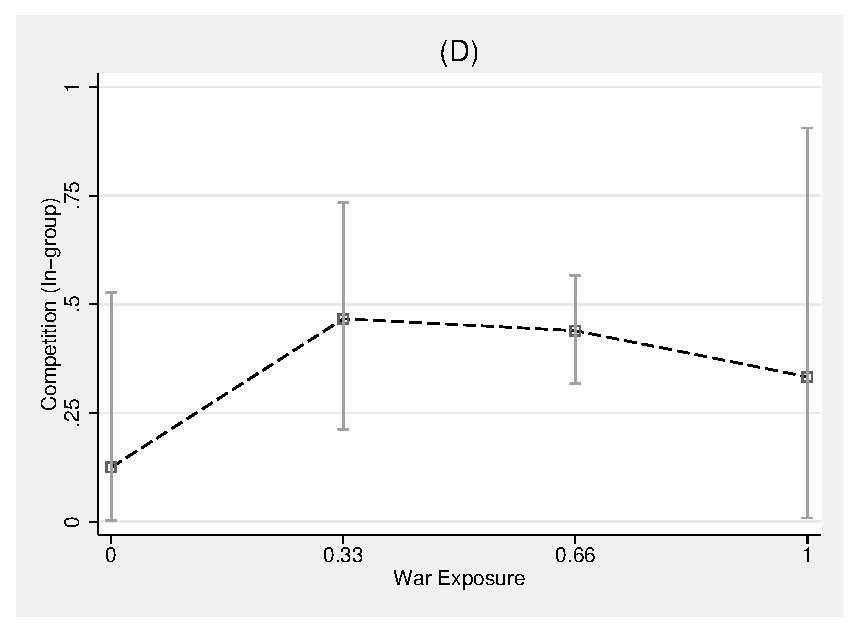
\includegraphics[width=0.8\linewidth]{"Outputs_anon/figures/f4_we_competition.eps"}
  \caption{Foul cards, competitiveness and exposure to violence}
  \label{fig:slf:we_competition}
  \subcaption*{\textit{Notes:} Competition and war expose: Panel A: Foul Card and war exposure for the entire sample; Panel B: willingness to compete and war exposure, entire sample; Panel C: willingness to compete and war exposure,  out-group only; Panel D: willingness to compete and war exposure, in-group only. All panels show binomial confidence intervals at the 95\% level.}
  \end{center}
\end{figure}

\begin{table}[p!]
\centering
\caption{Willingness to Compete}
\label{tab:slf:compete}
\begin{threeparttable}
  \singlespacing
  \small
  {
\def\sym#1{\ifmmode^{#1}\else\(^{#1}\)\fi}
\begin{tabularx}{0.9\textwidth}{Xl*{5}{c}}
\hline\hline
                    &\multicolumn{1}{c}{(1)}&\multicolumn{1}{c}{(2)}&\multicolumn{1}{c}{(3)}&\multicolumn{1}{c}{(4)}&\multicolumn{1}{c}{(5)}\\
                    &\multicolumn{1}{c}{Out-group}&\multicolumn{1}{c}{Out-group}&\multicolumn{1}{c}{In-group}&\multicolumn{1}{c}{In-group}&\multicolumn{1}{c}{Pooled}\\
\hline
                    &                     &                     &                     &                     &                     \\
Exposure to conflict&       0.485\sym{**} &       0.510\sym{**} &       0.274         &       0.266         &       0.500\sym{**} \\
                    &     (0.222)         &     (0.244)         &     (0.227)         &     (0.270)         &     (0.227)         \\
[0.5em]
Ingroup (d)         &                     &                     &                     &                     &       0.154         \\
                    &                     &                     &                     &                     &     (0.202)         \\
[0.5em]
Exposure to conflict × in-group&                     &                     &                     &                     &      -0.305         \\
                    &                     &                     &                     &                     &     (0.322)         \\
[0.5em]
Age                 &                     &       0.104         &                     &      -0.228         &      -0.132         \\
                    &                     &     (0.183)         &                     &     (0.160)         &     (0.114)         \\
[0.5em]
Age squared         &                     &    -0.00154         &                     &     0.00538         &     0.00336         \\
                    &                     &   (0.00416)         &                     &   (0.00362)         &   (0.00258)         \\
[0.5em]
Education Level     &                     &       0.171\sym{*}  &                     &       0.130         &       0.132\sym{**} \\
                    &                     &    (0.0986)         &                     &    (0.0834)         &    (0.0626)         \\
[0.5em]
Meals per day       &                     &     -0.0178         &                     &      -0.137         &     -0.0950         \\
                    &                     &     (0.110)         &                     &    (0.0975)         &    (0.0704)         \\
[0.5em]
Muslim (d)          &                     &       0.305\sym{***}&                     &     -0.0791         &      0.0384         \\
                    &                     &     (0.118)         &                     &     (0.150)         &     (0.104)         \\
[0.5em]
Mende (d)           &                     &     -0.0835         &                     &      0.0110         &     -0.0217         \\
                    &                     &     (0.148)         &                     &     (0.116)         &    (0.0889)         \\
[0.5em]
Played whole game (d)&                     &       0.405\sym{***}&                     &       0.191\sym{*}  &       0.204\sym{**} \\
                    &                     &     (0.136)         &                     &     (0.111)         &    (0.0847)         \\
[0.5em]
Self-declared skills&                     &      0.0206         &                     &      -0.222         &     -0.0592         \\
                    &                     &     (0.254)         &                     &     (0.299)         &     (0.191)         \\
[0.5em]
Scored (d)          &                     &      -0.267\sym{*}  &                     &      -0.125         &      -0.148         \\
                    &                     &     (0.147)         &                     &     (0.138)         &     (0.104)         \\
[0.5em]
Won the football game (d)&                     &       0.123         &                     &     -0.0747         &     0.00454         \\
                    &                     &     (0.135)         &                     &     (0.114)         &    (0.0848)         \\
[0.5em]
Left footed (d)     &                     &      -0.178         &                     &      -0.213\sym{*}  &      -0.204\sym{**} \\
                    &                     &     (0.140)         &                     &     (0.121)         &    (0.0908)         \\
\hline
N                   &          70         &          70         &          92         &          92         &         162         \\
Pseudo R-Squared    &       0.055         &       0.207         &       0.011         &       0.106         &       0.105         \\
\hline\hline
\end{tabularx}
}

  \begin{tablenotes}
    \footnotesize
    \item \textit{Notes:} robit marginal effects. Column 1 reports the univariate marginal effect of exposure to conflict on our experimental measure of willingness to compete towards the out-group (see Appendix I for variable definitions). Column 2 adds individual and football game related controls. Column 3 reports the univariate marginal effect of exposure to conflict on our experimental measure of willingness to compete towards the in-group. Column 4 adds individual and football game related controls. Column 5 reports the pooled marginal effect of exposure to conflict our experimental measure of willingness to compete, including individual and football game related controls, a group dummy, and an interaction term. Robust standard errors in parentheses. * p $<$ 0.10, ** p $<$ 0.05, *** p $<$ 0.01.
    \item
  \end{tablenotes}
\end{threeparttable}
\end{table}



\setcounter{table}{0}
\renewcommand{\thetable}{A\arabic{table}}

\begin{table}[htp]
  \caption{Willingness to Compete (out-group)}
  \label{tab:slf:compete_fe}
  Table A.1 Cannot be replicated using anonymized data.
\end{table}

\pagebreak

\begin{table}[htp]
  \caption{Willingness to Compete (out-group)}
  \label{tab:slf:compete_migrate}
\begin{threeparttable}[p!]

  \singlespacing
  %\renewcommand{\arraystretch}{0.6}
  % \tiny 
  % \scriptsize
  \footnotesize
  %\small
  % \normalsize
  {
\def\sym#1{\ifmmode^{#1}\else\(^{#1}\)\fi}
\begin{tabular}{l*{4}{c}}
\hline\hline
                    &\multicolumn{1}{c}{(1)}&\multicolumn{1}{c}{(2)}&\multicolumn{1}{c}{(3)}&\multicolumn{1}{c}{(4)}\\
                    &\multicolumn{1}{c}{\specialcell{Outgroup:\\Always in\\Kenema}}&\multicolumn{1}{c}{\specialcell{Outgroup:\\Migrated}}&\multicolumn{1}{c}{\specialcell{Outgroup:\\All}}&\multicolumn{1}{c}{\specialcell{Pooled}}\\
\hline
Self-select in tournament&                     &                     &                     &                     \\
War Exposure        &       0.635         &       0.895\sym{**} &       0.680\sym{**} &       0.678\sym{**} \\
                    &     (0.737)         &     (0.425)         &     (0.287)         &     (0.270)         \\
[1em]
ind\_alwaysken (d)   &                     &                     &      -0.258         &      0.0662         \\
                    &                     &                     &     (0.382)         &     (0.218)         \\
[1em]
int\_we\_ken          &                     &                     &      0.0510         &      -0.402         \\
                    &                     &                     &     (0.590)         &     (0.342)         \\
[1em]
ind\_age==20-24 (d)  &      -0.387         &      0.0397         &     -0.0783         &      -0.120         \\
                    &     (0.259)         &     (0.216)         &     (0.176)         &     (0.101)         \\
[1em]
ind\_age==25-29 (d)  &       0.147         &      -0.499\sym{***}&     -0.0346         &      0.0329         \\
                    &     (0.448)         &     (0.188)         &     (0.274)         &     (0.210)         \\
[1em]
ind\_age==30-34      &                     &                     &                     &                     \\
                    &                     &                     &                     &                     \\
[1em]
ind\_edu             &       0.249         &       0.497         &       0.228\sym{*}  &       0.169\sym{*}  \\
                    &     (0.211)         &     (0.421)         &     (0.129)         &    (0.0899)         \\
[1em]
Meals per day       &      -0.279         &     -0.0199         &      -0.127         &      -0.108         \\
                    &     (0.223)         &     (0.242)         &     (0.147)         &    (0.0781)         \\
[1em]
Muslim (d)          &       0.128         &      -0.150         &       0.207         &    -0.00967         \\
                    &     (0.329)         &     (0.301)         &     (0.160)         &     (0.120)         \\
[1em]
ind\_mende (d)       &      0.0252         &      -0.278         &      -0.146         &     -0.0225         \\
                    &     (0.384)         &     (0.275)         &     (0.161)         &    (0.0962)         \\
[1em]
Played whole game (d)&     0.00487         &       0.524\sym{*}  &       0.274\sym{*}  &       0.197\sym{**} \\
                    &     (0.276)         &     (0.283)         &     (0.164)         &    (0.0942)         \\
[1em]
Self-declared skills&       0.114         &       0.137         &      0.0501         &     -0.0146         \\
                    &     (0.474)         &     (0.407)         &     (0.288)         &     (0.205)         \\
[1em]
Scored (d)          &      -0.282         &      -0.539         &      -0.284\sym{*}  &      -0.217\sym{**} \\
                    &     (0.287)         &     (0.337)         &     (0.172)         &     (0.109)         \\
[1em]
Won the football game (d)&     -0.0882         &       0.210         &       0.140         &      0.0507         \\
                    &     (0.289)         &     (0.251)         &     (0.148)         &    (0.0923)         \\
[1em]
Left footed (d)     &                     &     -0.0339         &      -0.263\sym{**} &      -0.250\sym{***}\\
                    &                     &     (0.359)         &     (0.134)         &    (0.0915)         \\
[1em]
Exposure to conflict × in-group&                     &                     &                     &      -0.512         \\
                    &                     &                     &                     &     (0.335)         \\
[1em]
Ingroup (d)         &                     &                     &                     &       0.274         \\
                    &                     &                     &                     &     (0.201)         \\
\hline
N                   &          23         &          32         &          61         &         141         \\
R2                  &        0.16         &        0.30         &        0.20         &        0.11         \\
\hline\hline
\end{tabular}
}

  \begin{tablenotes}
    \footnotesize
    \item \textit{Notes:} Probit marginal effects. Column 1 reports the marginal effect of exposure to conflict on our experimental measure of willingness to compete towards the out-group (see Appendix I for variable definitions), including individual and football game related controls, for the subsample of respondents who were born and had never moved out of Kenema district. Column 2 presents the outcomes for the remaining subsample, born elsewhere or temporarily out-migrated from Kenema district during the conflict. Column 3 reports the marginal effect of exposure to conflict on our experimental measure of willingness to compete towards the out-group, including individual and football game related controls, and a variable capturing the absence of temporary out-migration. Column 4 presents the outcome for the pooled sample (in-group and out-group). Robust standard errors in parentheses. * p $<$ 0.10, ** p $<$ 0.05, *** p $<$ 0.01.
    \item
  \end{tablenotes}
\end{threeparttable}
\end{table}

\pagebreak

\begin{table}[htp]
  \caption{Willingness to Compete (out-group)}
  \label{tab:slf:compete_disp}
\begin{threeparttable}[p!]

  \singlespacing
  %\renewcommand{\arraystretch}{0.6}
  % \tiny 
  % \scriptsize
  %\footnotesize
  \small
  % \normalsize
  {
\def\sym#1{\ifmmode^{#1}\else\(^{#1}\)\fi}
\begin{tabular}{l*{4}{c}}
\hline\hline
                    &\multicolumn{1}{c}{(1)}&\multicolumn{1}{c}{(2)}&\multicolumn{1}{c}{(3)}&\multicolumn{1}{c}{(4)}\\
                    &\multicolumn{1}{c}{Self-select in tournament}&\multicolumn{1}{c}{Self-select in tournament}&\multicolumn{1}{c}{Self-select in tournament}&\multicolumn{1}{c}{Self-select in tournament}\\
\hline
Self-select in tournament&                     &                     &                     &                     \\
War Exp. incl. displacement&       0.916\sym{***}&                     &                     &                     \\
                    &     (0.339)         &                     &                     &                     \\
[1em]
Exposure to conflict&                     &       0.882\sym{**} &       0.974\sym{**} &       0.690\sym{**} \\
                    &                     &     (0.392)         &     (0.447)         &     (0.322)         \\
[1em]
ind\_age==20-24 (d)  &       0.049         &       0.080         &       0.221         &       0.086         \\
                    &     (0.212)         &     (0.248)         &     (0.283)         &     (0.212)         \\
[1em]
ind\_age==25-29      &                     &                     &                     &                     \\
                    &                     &                     &                     &                     \\
[1em]
ind\_edu             &       0.191         &       0.062         &      -0.069         &       0.205         \\
                    &     (0.150)         &     (0.173)         &     (0.207)         &     (0.128)         \\
[1em]
Meals per day       &      -0.074         &       0.132         &       0.370         &      -0.031         \\
                    &     (0.154)         &     (0.205)         &     (0.238)         &     (0.115)         \\
[1em]
Muslim (d)          &       0.501\sym{***}&                     &                     &       0.495\sym{***}\\
                    &     (0.088)         &                     &                     &     (0.073)         \\
[1em]
ind\_mende (d)       &      -0.251         &      -0.412         &      -0.397         &      -0.210         \\
                    &     (0.186)         &     (0.256)         &     (0.276)         &     (0.169)         \\
[1em]
Played whole game (d)&       0.396\sym{**} &       0.554\sym{**} &       0.660\sym{***}&       0.422\sym{***}\\
                    &     (0.183)         &     (0.217)         &     (0.236)         &     (0.105)         \\
[1em]
Self-declared skills&       0.278         &       0.257         &      -0.026         &       0.226         \\
                    &     (0.339)         &     (0.366)         &     (0.442)         &     (0.327)         \\
[1em]
Scored (d)          &      -0.421\sym{***}&      -0.247         &      -0.010         &      -0.393\sym{***}\\
                    &     (0.144)         &     (0.266)         &     (0.408)         &     (0.147)         \\
[1em]
Won the football game (d)&       0.383\sym{**} &       0.382\sym{**} &                     &       0.328\sym{**} \\
                    &     (0.159)         &     (0.166)         &                     &     (0.161)         \\
[1em]
Left footed (d)     &      -0.326\sym{**} &      -0.413\sym{***}&      -0.500\sym{***}&      -0.300\sym{**} \\
                    &     (0.142)         &     (0.154)         &     (0.107)         &     (0.135)         \\
[1em]
Constant            &                     &                     &                     &                     \\
                    &                     &                     &                     &                     \\
\hline
N                   &          49         &          40         &          35         &          49         \\
R2                  &       0.264         &       0.289         &       0.296         &       0.253         \\
\hline\hline
\multicolumn{5}{l}{\footnotesize Marginal effects; Standard errors in parentheses}\\
\multicolumn{5}{l}{\footnotesize  (d) for discrete change of dummy variable from 0 to 1}\\
\multicolumn{5}{l}{\footnotesize \sym{*} \(p<0.10\), \sym{**} \(p<0.05\), \sym{***} \(p<0.01\)}\\
\end{tabular}
}

  \begin{tablenotes}
    \footnotesize
    \item \textit{Notes:} Probit marginal effects. Column 1 reports the marginal effect of exposure to conflict on our experimental measure of willingness to compete towards the out-group (see Appendix I for variable definitions), including individual and football game related controls, were the exposure to conflict includes a dummy for forced displacement as additional measure of victimization. Column 2 includes football match fixed effects. Column 3 includes team fixed effects. Column 4 clusters standard errors at the team level. 7 Observations dropped in (3) due to quasi-separation issues related to small group fixed effects. Robust standard errors in parentheses. * p $<$ 0.10, ** p $<$ 0.05, *** p $<$ 0.01.
    \item
  \end{tablenotes}
\end{threeparttable}
\end{table}

\pagebreak

\begin{table}[htp]
  \caption{Willingness to Compete (out-group)}
  \label{tab:slf:compete_abl}
\begin{threeparttable}[p!]

  \singlespacing
  %\renewcommand{\arraystretch}{0.6}
  % \tiny 
  % \scriptsize
  %\footnotesize
  \small
  % \normalsize
  {
\def\sym#1{\ifmmode^{#1}\else\(^{#1}\)\fi}
\begin{tabular}{l*{4}{c}}
\hline\hline
                    &\multicolumn{1}{c}{(1)}&\multicolumn{1}{c}{(2)}&\multicolumn{1}{c}{(3)}&\multicolumn{1}{c}{(4)}\\
                    &\multicolumn{1}{c}{Self-select in tournament}&\multicolumn{1}{c}{Self-select in tournament}&\multicolumn{1}{c}{Self-select in tournament}&\multicolumn{1}{c}{Self-select in tournament}\\
\hline
Self-select in tournament&                     &                     &                     &                     \\
War Exposure        &       0.516\sym{**} &       0.535\sym{**} &       0.470\sym{*}  &       0.495\sym{*}  \\
                    &     (0.243)         &     (0.250)         &     (0.253)         &     (0.256)         \\
[1em]
Standardized values of (switch)     &      0.0262         &                     &                     &      0.0179         \\
                    &    (0.0723)         &                     &                     &    (0.0715)         \\
[1em]
Expected performance&                     &       0.489         &                     &       0.467         \\
                    &                     &     (0.580)         &                     &     (0.591)         \\
[1em]
ballshit            &                     &                     &     -0.0230         &     -0.0233         \\
                    &                     &                     &    (0.0386)         &    (0.0396)         \\
[1em]
Age                 &      0.0992         &      0.0872         &      0.0889         &      0.0699         \\
                    &     (0.185)         &     (0.186)         &     (0.183)         &     (0.188)         \\
[1em]
Age squared         &    -0.00145         &    -0.00126         &    -0.00117         &   -0.000842         \\
                    &   (0.00420)         &   (0.00421)         &   (0.00417)         &   (0.00427)         \\
[1em]
Education Level     &       0.172\sym{*}  &       0.159         &       0.180\sym{*}  &       0.169         \\
                    &    (0.0988)         &     (0.101)         &     (0.101)         &     (0.104)         \\
[1em]
Meals per day       &     -0.0191         &     -0.0299         &     -0.0198         &     -0.0318         \\
                    &     (0.111)         &     (0.109)         &     (0.110)         &     (0.111)         \\
[1em]
Muslim (d)          &       0.306\sym{**} &       0.311\sym{***}&       0.315\sym{***}&       0.320\sym{***}\\
                    &     (0.119)         &     (0.118)         &     (0.117)         &     (0.117)         \\
[1em]
Mende (d)           &     -0.0966         &     -0.0740         &     -0.0828         &     -0.0821         \\
                    &     (0.147)         &     (0.152)         &     (0.149)         &     (0.150)         \\
[1em]
Played whole game (d)&       0.403\sym{***}&       0.373\sym{**} &       0.429\sym{***}&       0.397\sym{***}\\
                    &     (0.138)         &     (0.146)         &     (0.140)         &     (0.151)         \\
[1em]
Self-declared skills&      0.0257         &     -0.0621         &      0.0430         &     -0.0318         \\
                    &     (0.256)         &     (0.275)         &     (0.261)         &     (0.283)         \\
[1em]
Scored (d)          &      -0.268\sym{*}  &      -0.253         &      -0.288\sym{**} &      -0.277\sym{*}  \\
                    &     (0.148)         &     (0.155)         &     (0.141)         &     (0.146)         \\
[1em]
Won the football game (d)&       0.131         &       0.114         &       0.146         &       0.143         \\
                    &     (0.137)         &     (0.134)         &     (0.141)         &     (0.143)         \\
[1em]
Left footed (d)     &      -0.187         &      -0.156         &      -0.212         &      -0.199         \\
                    &     (0.140)         &     (0.150)         &     (0.143)         &     (0.150)         \\
\hline
N                   &          70         &          70         &          70         &          70         \\
R2                  &       0.209         &       0.215         &       0.211         &       0.219         \\
\hline\hline
\multicolumn{5}{l}{\footnotesize Marginal effects; Standard errors in parentheses}\\
\multicolumn{5}{l}{\footnotesize  (d) for discrete change of dummy variable from 0 to 1}\\
\multicolumn{5}{l}{\footnotesize \sym{*} \(p<0.10\), \sym{**} \(p<0.05\), \sym{***} \(p<0.01\)}\\
\end{tabular}
}

  \begin{tablenotes}
    \footnotesize
    \item \textit{Notes:} Probit marginal effects. Column 1 reports the marginal effect of exposure to conflict on our experimental measure of willingness to compete towards the out-group (see Appendix I for variable definitions), including individual and football game related controls, and our experimental measure of risk preferences. Column 2 includes expected relative performance, standardized between 0 (the worst) and 1 (the best). Column 3 includes actual performance in terms of the number of balls on target (standardized). Column 4 includes all three measures risk preferences, performance expectation, and skills. Robust standard errors in parentheses.  * p $<$ 0.10, ** p $<$ 0.05, *** p $<$ 0.01.
    \item
  \end{tablenotes}
\end{threeparttable}
\end{table}

\clearpage
\bibliographystyle{chicago}
%path to .bib file (e.g. automatically exported by mendeley) DO NOT include the file extension!
\bibliography{Thesis-Football}

\end{document}